\documentclass[journal]{IEEEtran}
\usepackage{cite}
\usepackage[dvips]{graphicx}
\begin{document}
%Continuous group index and dispersion measurements in slow light corrugated waveguides
\title{Optical phase characterization of integrated photonic devices}
\author{J.~Matres,~G.~C.~Ballesteros,~S.~Mas,~A.~Brimont,~P.~Sanchis,~J.~Mart\'i~and~C.~J.~Oton}
%\markboth{IEEE PHOTONICS TECHNOLOGY LETTERS}%
%{Shell \MakeLowercase{\textit{et al.}}: Continuous group index and dispersion measurements in slow light corrugated waveguides}

\maketitle


\begin{abstract}
%We use wavelength-continuous phase measurements to characterize the parameters of an optical ring-resonator and measure the group index in a slow light corrugated waveguide. The setup is based on an heterodyne Mach Zehnder interferometry technique, as the MZI is in an external setup, any simple waveguide can be easily characterized.

We propose a relatively simple experimental setup capable of accurately characterizing the optical phase response of an integrated photonic circuit. The setup is based on a phase-noise reduction scheme using an external  heterodyne Mazch-Zehnder interferometer. In particular, we characterize the phase response of different silicon photonic components: undercoupled and overcoupled ring resonators, and a corrugated  waveguide.



\end{abstract}

%We present a wavelength continuous phase measurement technique that allow us to characterize structures based on an heterodyne Mach Zehnder interferometry technique. As the MZI is in an external setup, any simple waveguide can be easily characterized. Group index and dispersion is derived from the phase measurements in slow light corrugated waveguides and the same technique is used to distinguish under-coupled and over-coupled micro-ring resonators. The method is immune to thermal fluctuations thanks to a counter-propagating reference beam. Conventional discrete Mach-Zehnder-Interferometer group index measurements are also shown for comparison with our technique.


\section{Introduction}
%\noindent Silicon photonics has recently emerged as a viable technology for integrated photonic devices. Micro-ring resonators are elements which are simple to fabricate and are used for devices such as optical filters, \cite{Little1998b}, sensors, \cite{Dumon2004}  modulators, \cite{Almeida2004b} etc. The quality factor is usually the parameter that determines the performance of the device; in these devices one of the key factors is achieving critical coupling, in which the internal losses in the ring are equal to the coupling losses, making the transmitted power 0; however, in most cases it is hard to determine whether the ring resonators are under or over-coupled. In this paper, we propose a characterization technique to differentiate both cases monitoring the phase evolution versus wavelength.

In the last years, integrated optics has seen a remarkable development thanks to technological advances but also because its recent trend towards standarization.
The main advantage of photonic integrated circuits is that one can build a extremely complex systems with hundreds of components on a very small footprint and at a very low cost per device.
System design usually requires scattering parameters of single components in order to simulate a complex system.
The measurement of these parameters requires the characterization of the phase response of the element.
This is not straightforward, as under normal circumstances phase noise prevents simple interferometric measurements using for example a Mach-Zehnder interferometer (MZI).

Several techniques have been proposed to alleviate phase noise problems in the fringe characterization of the measurement.
However these techniques usually require very precise temperature control, or very fast tuning rates [REF].
Commercial devices sensitive to phase are typically called optical vector network analyser (OVNA).
These instruments usually employ tunable lasers with tuning speeds of xxxx nm/s.
In this work, we present a relatively simple setup which allows accurate and continuous phase response of the system by using an ordinary tunable laser with tuning speeds in the order of few nm/s. The cancellation of phase noise is carried out by employing a counter-propagating reference beam at fixed wavelength.
This idea was applied in Ref. [REF SARA] to characterize chromatic disperion in waveguides with different geometries.
This paper shows that the setup can be used to characterize the phase response of different building blocks, in particular, silicon microring resonators and corrugated waveguides. In the former, the measurement allowed us to distinguish undercoupling from overcoupling conditions.
In the latter, a detailed plot of the group index of the corrugation can be obtained from a single segment of waveguide without the need of integrated MZIs and fringe spacing calculations.


\section{Experimental setup}

The experimental setup is shown in Fig. xxxxxx.
It constists of a fiber-based MZI, where each branch has a an acousto-optic modulator (AOM) which acts as a frequency shifter.
The frequency shift applied to each branch is slightly different, in order to make it heterodyne (in our experiment, the difference was 40kHz), which produces a beating pattern which can be measured with a lock-in amplifier. The phase of these beatings with respect to the RF generators provides the phase of the system, but this is also affected by thermal phase noise, which can be as high as several radians per second. This noise would make unfeasable a phase characterization with a laser with tuning speed in the order of few nm/s. To cancel the phase noise, a reference counter-propagating beam at a fixed wavelength was introduced from the opposite end.
This signal produces another beating pattern which can be detected with a second photodiode, amplified, and used as a reference for the lock-in amplifier.
As thermal fluctuations equally affect both beams, they cancel out, and only the wavelength-dependent phase variations are measured. An optical delay line (ODL) is also introduced in one branch in order to keep the interferometer balanced when different device lengths are measured. 


If the building block to characterize is placed in series with other elements, (couplers, connecting waveguides, tapers, etc.) the measurement requires a reference sample with the same elements, but without the component under test (e.g. the corrugated waveguide). Before each sweep is launched, the MZI must be balanced in order to avoid too steep slopes in the phase dependence on $\omega$.
In addition, it is convenient to set the wavelength of the counter-propagating reference beam, $\omega_0$, approximately in the middle of the sweep in order to get small The reference sweep provides the system response, which must be subtracted from the measurement which includes the component under test. 

Mathematically, the phase dependence obtained with the lock-in, after subtracting the system response, becomes:


\begin{equation}
\phi(\omega)=\phi_{c}(\omega)-\frac{\omega\Delta L}{c}
\label{eq:response}
\end{equation}
where $\phi$ is the measured phase, $\phi_{c}$ the phase introduced by the component under test, $\Delta L$ the extra length introduced in the ODL to balance the MZI with respect to the reference measurement, and $c$ the speed of light in vacuum. It can be demonstrated [REF SARA] that if the component under test has a length $L_{c}$, then the the group index of the component is precisely:

\begin{equation}
n_{g} = \frac{\Delta L}{L_{c}}
\label{eq:group_index}
\end{equation}
The balancing of the MZI is carried out by minimizing the slope of the phase versus wavelength. A slope equal to zero at a certain wavelength corresponds to perfect balancing, so the group index of the component under test can be extracted. Finally, its dependence on wavelength is extracted from its variation versus wavelength when the sweep is acquired.

It is worth mentioning that as the lock-in can simultaneously provide the phase and the amplitude of the output, a complete phase and amplitude characterization is possible with the setup in one single sweep. Moreover, amplitude noise due to gradual slight misalignments can also be cancelled out by normalizing with the amplitude of the reference signal.



\section{Experimental results}

\subsection {Ring resonators}

[Aqui lo cedo a ti para que continúes tu. Yo haria una introduccion a los rings bastante mas breve, dejando solo las ecuaciones mas importantes]

[La Fig. 1 no hace falta, quiza podria quedar bien una foto sem del anillo, si la tenemos por ahi, del mismo modo que mostramos una foto sem de la corrugada]



An optical ring resonator is a structure formed connecting the input of a directional coupler to one of the outputs. When light of a certain wavelength is coupled to the ring, constructive or destructive interference is generated in the multiple turns, so only the wavelengths that satisfy the resonance condition remain inside the ring (Eq.~\ref{eq:resonanceCondition}), which are multiples of the ring length. The rest of the wavelengths accumulate different phase shifts along the ring and interfere destructively. 

% Therefore no light is at the output when the condition of resonance is present, having a transmission minimum for those wavelengths.
% An optical ring resonator is a structure formed connecting the input of a directional coupler to one of the outputs. When light of a certain wavelength is coupled to the ring constructive or destructive interference is generated in the multiple turns along the ring, so only the wavelengths that satisfy the resonance condition remain (Eq.~\ref{{eq:resonanceCondition}}), which are those having a wavelength corresponding to integer multiples of the length of the ring, the other accumulate different phase shift and add up destructively. Therefore no light is at the output when the condition of resonance is present, having a transmission minimum for those wavelengths.
% which are those having a wavelength corresponding to integer multiples of the length of the ring

\begin{equation}
	n_{eff}  L = m \lambda_i
	\label{eq:resonanceCondition}
\end{equation} 

\begin{figure}[htb]
    \centering
    \includegraphics[width=2.5in]{ring}
    \caption{Schematic of a ring resonator. k: coupling, t: transmission, A: attenuation and phase shift per turn inside the ring.}
    \label{fig:ringSchematic}
\end{figure}


Ring resonators are very useful components for filtering, multiplexing, switching and modulating. The most important parameters of the rings are the free spectral range (FSR), the extinction ratio (ER), and the width of the resonance (FWHM), related to the quality factor (Q) and finesse of the resonance ($F$). These parameters depend not only in design but also manufacturing tolerances.

\begin{equation}
	FSR=\frac{\lambda_{res}^2}{n_gL}
\end{equation} 

\begin{equation}
	Q=mF=m\frac{FSR}{FWHM}
\end{equation} 

The transmission equation of a ring can be easily obtained. If we consider an input field $E_{in}$, the first contribution at the output is $E_{in} t$ being $t$ the transmission in the coupler (Fig.~\ref{fig:ringSchematic}). The second contribution ($-E_{in} k^2$) is attenuated by the ring losses ($A$), two coupling coefficients ($k^2$) and a negative sign due to the $\pi/2$ shift to enter the ring and another $\pi/2$ phase shift to go back into the waveguide.


% The transmission equation of a ring can be easily obtained. If we consider an input field $E_{in}$, the first contribution at the output  $E_{in} t$ being $t$ the transmission in the coupler (Fig.~\ref{fig:ringSchematic}). The second contribution will be the attenuated by the ring losses ($A$), two coupling coefficients ($k^2$) and a negative sign due to the $\pi/2$ shift to enter the ring and another $\pi/2$ phase shift to go back into the waveguide.

\begin{equation}
	E_{out}=E_{in}[t-k^2A-k^2tA^2 + \ldots]
\end{equation} 

\begin{equation}
	E_{out}/E_{in}=t-k^2A[1+tA + (tA)^2 +  \ldots]
\end{equation} 

Where the sum of the infinite terms of a geometric progression of common ratio $tA<1$ is $ S_\infty = \frac{1}{1-tA} $

\begin{equation}
	E_{out}/E_{in}=t-k^2A\frac{1}{1-tA}
\end{equation} 

\begin{equation}
	E_{out}/E_{in}=\frac{t-t^2A-K^2A}{1-tA}
\end{equation} 

And we know that $k^2+t^2=1$, so we can substitute $k^2=1-t^2$:

\begin{equation}
	E_{out}/E_{in}=\frac{t-A}{1-tA}
\label{eq:transmissionRing}
\end{equation}

Where $A=\alpha e^{j\phi}$, which in resonance $\phi=\beta L=2\pi \frac{ n_{eff}}{\lambda} 2 \pi R= 0,2\pi,4\pi,\ldots$, we only have the losses term ($A=\alpha$). Notice that usually losses are given in dB/cm, $L{ring}(dB/cm)=20log_{10}(A)/(2\pi R)$, where R is the ring radius in centimeters.


Depending on the relation between the coupling coefficient and the losses, the ring can be:

\begin{itemize}
 \item \textbf{Critically coupled ($t=A$):}  there is no transmission as eq.~\ref{eq:transmissionRing} goes to zero. The same energy that goes through the coupler goes in and out of the ring with a $\pi$ phase shift so there is a destructive interference at the output.
 
 \item \textbf{Under-coupled ($k<A,t>A$):}  more energy goes through the coupler than inside the ring. Very little phase shift is produced in the resonances. Small valleys are seen in transmission because even with the ring is filled with multiples of the resonance wavelength, low power has been coupled into the ring, so the resonances make small changes in phase and amplitude.	
 
 \item \textbf{Over-coupled ($k>A,t<A$):}  more energy goes inside the ring than through the coupler. Each of the resonances causes a $2\pi$ phase shift when sweeping the wavelength. Before entering the resonant regime light goes through the coupler and not into the ring (0 rad phase shift), with the ring in resonance most of the energy goes in and out of the ring, so the effective phase shift is $\pi$ rad. Finally when we leave the resonant regime there is another $\pi$ rad phase shift.
\end{itemize}

\begin{figure}[htb]
    \centering
    \includegraphics[width=3.5in]{ringTesis}
    \caption{Spectral amplitude (top) and phase (bottom) simulations of a 20~$\mu$m ring resonator for different coupling conditions. Notice that only monitoring the phase we can distinguish the under-coupled from the over-coupled ring.}
    \label{fig:ringDifferentCoupling}
\end{figure}

In paper \cite{McKinnon2009} a method is developed for extracting the coupling and loss coefficients. However the formulas used do not distinguish which coefficient is loss and which is coupling. As we can see in Fig.~\ref{fig:ringDifferentCoupling} monitoring the phase we clearly distinguish an under-coupled ring from an over-coupled, even when the transmission response is exactly the same. In this paper we propose using also the phase information to extract the parameters of the ring resonator.


% fitting the phase of the ring resonators as a more robust measurement than using the transmission.

% the phase of the ring resonators as a more robust measurement than using the transmission.


% , which is more affected by .
% it is imposible to distinguish 
% The main problem in trying to obtain

\section{Optical phase measurement technique}
[Esta seccion ya se podria quitar, porque esta ya introducida antes]

We use acousto-optic modulators to create frequency shifts of 80 and 80.04~MHz. Beating those, creates a 40~KHz signal in the photo-diode, and the lock-in amplifier monitors its phase. We use the counter-propagating beatings of a fixed laser as reference signal in the lock-in; this way we reduce thermal noise. An optical delay line is used for path balancing the interferometer (See Fig.~\ref{fig:dispersionSetup}). The phase evolution is measured when changing the laser wavelength.


If we expand the propagation constant in Taylor series:

\begin{equation}
	\beta(\omega)=n(\omega)\frac{\omega}{c}=\beta_0+\beta_1(\omega-\omega_0)+\frac{1}{2}\beta_2(\omega-\omega_0)^2 + \frac{1}{6}\beta_3(\omega-\omega_0)^3 + \ldots
\end{equation}


We can extract the group index ($n_g$) from the first derivative of the phase:

\begin{equation}
	\beta_1=1/Ld\phi/d\omega=n_g/c
\end{equation}

And the dispersion parameter (D) is related with $\beta_2$ as:

\begin{equation}
	D=-\frac{2\pi c}{\lambda^2}\frac{d}{d\omega}(\frac{1}{v_g})=-\frac{2\pi c}{\lambda^2}\beta_2
\end{equation}


\begin{figure}[htb]
	\centering
	\includegraphics[width=3.5in]{dispersion3}
	\caption{Optical phase characterization setup. AOM: acousto-optic modulator. Dashed lines are electrical connections. In light green color is the tunable laser whose phase is monitored in the lock-in amplifier. In dark blue is the counter-propagating beam used as a reference in the Lock-in amplifier to compensate thermal fluctuations.}
	\label{fig:dispersionSetup}
\end{figure}



\section{Ring resonators characterization}
%Phase measurements to distinguish between under-coupled and over-coupled 
%On the other hand, $445 \times 220$~nm Si strip waveguides were fabricated with 20~$\mu$m ring resonators coupled 200 and 275~nm to the waveguides. In all cases t
% Phase measurements allow us to clearly distinguish between under-coupled and over-coupled ring resonators. 
% Critical coupling condition is achieved when the internal losses in the ring are equal to the coupling losses, making the transmitted power 0.
% However, with the transmission spectra we can not determine if the rings are under, over or critically coupled. 
% Monitoring the phase response of the resonances we clearly see that under-coupled rings accumulate $2\pi$ phase shifts (Fig.~\ref{fig:undercoupled}) while over-coupled have phase rebounds in each resonance (Fig.~\ref{fig:overcoupled}).


First we characterized the amplitude response of the rings sweeping the wavelength of a tunable laser at the input and monitoring the output power with a power meter. Then, using setup shown in Fig.~\ref{fig:dispersionSetup} we monitored the phase evolution in the same wavelength range. Finally, amplitude and phase responses were normalized by a waveguide without ring and fitted to the ring transfer function $H(\omega)=E_{in}/E_{out}=\mathrm{amplitude}\cdot e^{j\cdot \mathrm{phase}} = \frac{t-A}{1-tA}$ . As we can see in Fig.~\ref{fig:undercoupled} we clearly see that under-coupled rings accumulate $2\pi$ phase shifts while over-coupled have phase rebounds in each resonance as in Fig.~\ref{fig:overcoupled}. 



% % Combining both amplitude and phase transfer function $H(\omega)=E_{in}/E_{out}=\mathrm{amplitude}\cdot e^{j\cdot \mathrm{phase}}$ after normalizing them by a waveguide without ring, we fitted them to the ring transfer function (eq.~\ref{eq:transmissionRing}). As we can see in Fig.~\ref{fig:undercoupled} we clearly see that under-coupled rings accumulate $2\pi$ phase shifts while over-coupled have phase rebounds in each resonance as in Fig.~\ref{fig:overcoupled}.



% Then we measured the phase evolution in the lock-in amplifier when changing the wavelength. Both responses were normalized by a waveguide without ring, combined as $H(\omega)=E_{in}/E_{out}=\mathrm{amplitude}\cdot e^{j\cdot \mathrm{phase}}$, fitting the complex $H(\omega)=E_{in}/E_{out}$ to the ring transfer function (eq.~\ref{eq:transmissionRing}). In Fig.~\ref{fig:undercoupled} we clearly see that under-coupled rings accumulate $2\pi$ phase shifts while over-coupled have phase rebounds in each resonance as in Fig.~\ref{fig:overcoupled}.
% First we characterized the linear response of the rings sweeping the wavelength of a tunable laser at the input and monitoring the output power with a power meter. Then we measured the phase evolution in the lock-in amplifier when changing the wavelength. Both responses were normalized by a waveguide without ring, fitting the complex $H(\omega)=E_{in}/E_{out}$ to the ring transfer function (eq.~\ref{eq:transmissionRing}). In Fig.~\ref{fig:undercoupled} we clearly see that under-coupled rings accumulate $2\pi$ phase shifts while over-coupled have phase rebounds in each resonance as in Fig.~\ref{fig:overcoupled}.
     
\begin{figure}[htb]
\centerline{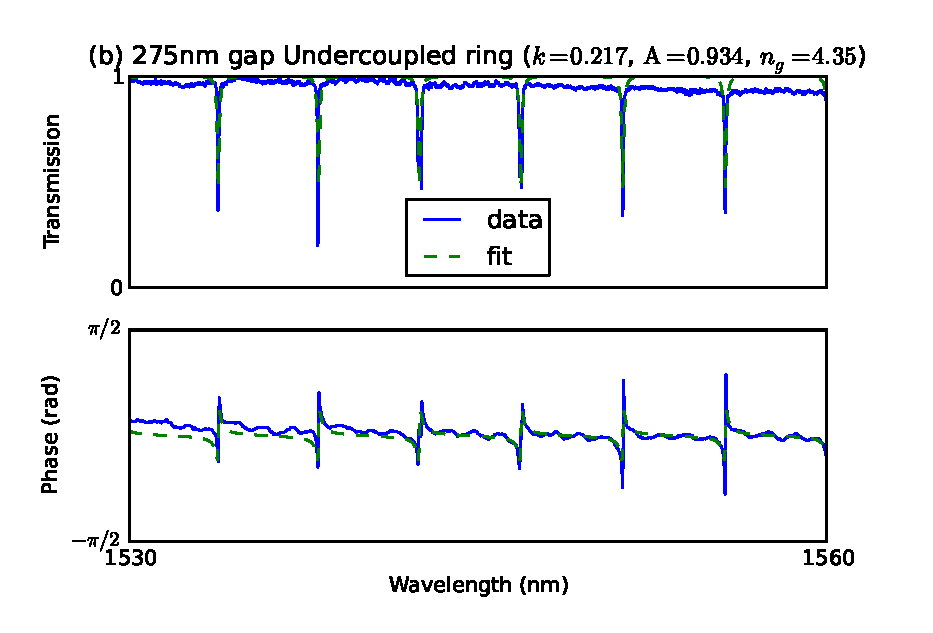
\includegraphics[width=9cm]{r20g275TE_fitPhaseAmp}}
\caption{TE 20~$\mu$m radius and 275~nm gap ring spectrum measurement (--) and fit (-~-) for a coupling coefficient $k=0.22$, $\mathrm{losses=47~dB/cm}$ and effective index $n_{eff}=4.35$.}
\label{fig:undercoupled}
\end{figure}

%[ k= 0.21659667  A= 0.93423178  neff= 4.35316758] -47.022906404 dB/cm

% (blue dotted curves)
% \caption{TE ring with 20~$\mu$m radius and 275~nm gap. Top: transmission spectra measured with a tunable laser at the input and a power meter at the output. Bottom: Phase evolution monitored in the lock-in amplifier when changing the wavelength. In light green dashed line is the response of a waveguide without ring.}
\begin{figure}[htb]
\centerline{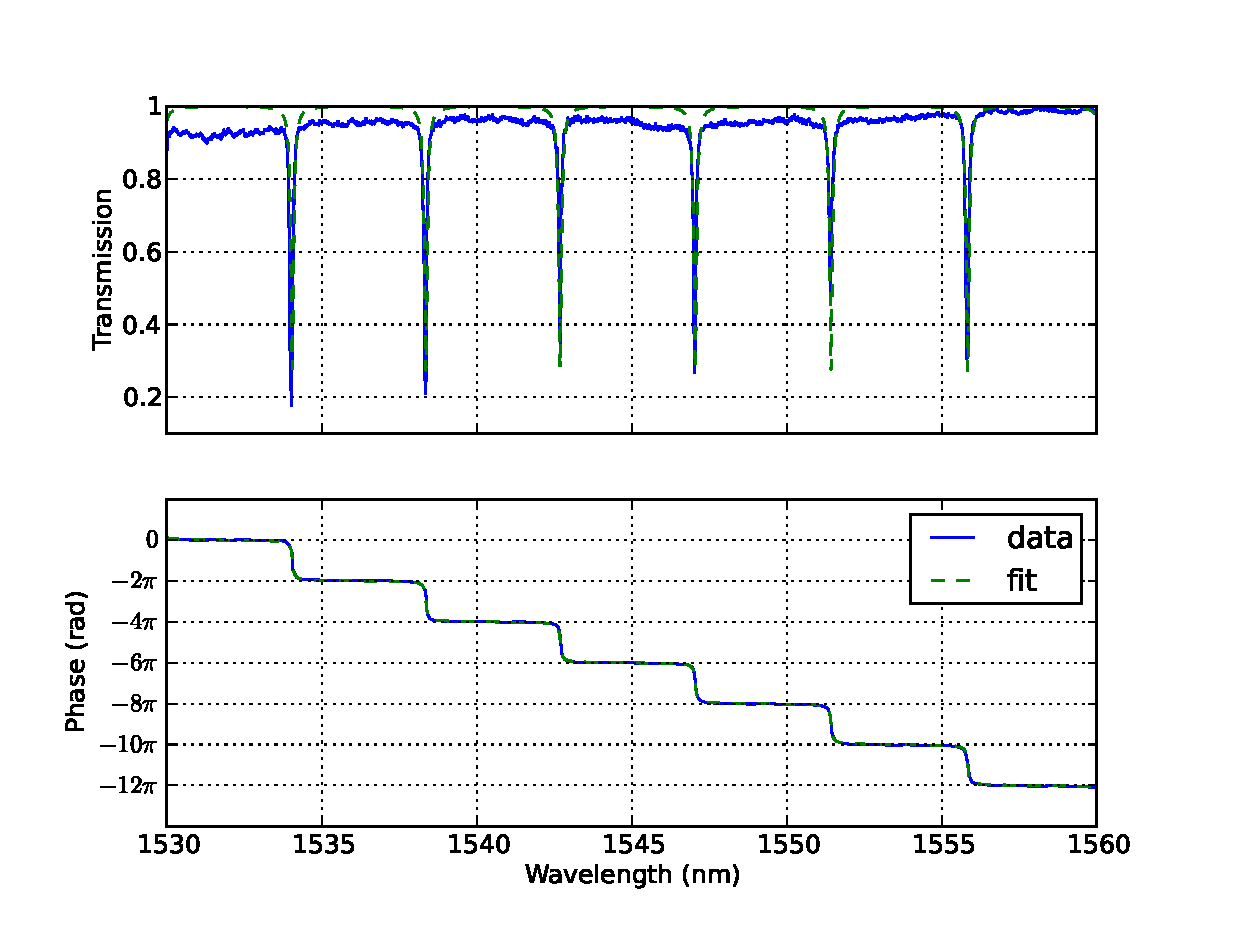
\includegraphics[width=9cm]{r20g200TE_fitPhaseAmp}}
\caption{TE 20~$\mu$m radius and 200~nm gap ring spectrum measurement (--) and fit (-~-) for a coupling coefficient $k=0.35$, $\mathrm{losses=25~dB/cm}$ and effective index $n_{eff}=4.36$}
\label{fig:overcoupled}
\end{figure}

% [k = 0.35048909  0.96328564  4.35909895] -25.8545799362 dB/cm
% in Fig.~\ref{fig:dispersionSetup} setup


\subsection{Slow light corrugated waveguides}

[Esto seria tambien una subsection. Yo aqui quitaria tambien la figura 7. Y la Figura 9 podria introducirse como un inset de la 8, o bien antes de la 8. Asi dices primero el metodo tradicional de medir n grupo, citando un par de papers, y luego muestras la figura 8.
Por cierto, en la 8 la parabola me parece un poco demasiado perfecta para ser real, es porque hiciste un fit polinomial a orden demasiado bajo? Cómo quedaría sin fit, o con fit a un orden más alto? En cualquier caso, puedes también restringir lo que muestras a la zona donde hay puntos verdes.]

% The refractive index increase in periodic structures is a phenomena known as slow light. This enhancement in light-matter interaction has been used to enhance nonlinear effects~\cite{Vlasov2005,Li2011,Monat2010}.
% 
% In~\cite{Mas2012}, a technique to determine the group index ($n_g$), group velocity dispersion (GVD) and dispersion slope ($\beta_3$) was presented. With this technique and dispersion tailoring designs~\cite{Turner2006}, high nonlinear waveguides could be designed for different applications such as all-optical modulators~\cite{Almeida2004b}, wavelength converters~\cite{Lee2009}, demultiplexers~\cite{Koos2009}, format converters~\cite{Astar2010}, etc.

In \cite{Dulkeith2006} dispersion and group index is characterized both for TE and TM waveguides. It is measured with an unbalanced integrated Mach Zehnder interferometer. So only a discrete amount of points is obtained, deriving group index and dispersion measurements from them. On the other hand, our technique using a phase sensitive setup allows a more accurate direct and continuous measurement with as high resolution as necessary.

The measured corrugated waveguides were fabricated using the EPIXFAB platform, processed from SOI wafers with 220~nm Si thickness, patterned with deep-UV lithography and covered with silica after the etching process. They were designed with a nearly constant group index in a relatively broad wavelength range (from 1560 to 1610~nm), achievable by patterning circular holes onto the wide section of the waveguide as in~\cite{Brimont2010} (See Fig.~\ref{fig:sem}). Transverse-electric polarization (TE) light was coupled through grating couplers.

\begin{figure}[htb]
	\centering
	\includegraphics[width=2.5in]{corr}	
	\caption{SEM image of the corrugated waveguide.}
	\label{fig:sem}
\end{figure}

% In \cite{Dulkeith2006} dispersion and group index is characterized both for TE and TM waveguides. It is measured with an unbalanced integrated Mach Zehnder interferometer. So only a discrete amount of points is obtained, deriving group index and dispersion measurements from them. On the other hand, a technique using a phase sensitive setup would allow to  obtain an accurate, direct and continuous measurement with as high resolution as needed.

\subsection{Group index measurements}
One corrugated waveguide was 27~$\mu$m long and the other 450~$\mu$m. Subtracting the phase evolutions of the 450~$\mu$m and 27~$\mu$m we obtain the phase evolution of a 423~$\mu$m waveguide without the system response as we can see in Fig.~\ref{fig:phaseEvolution}.


\begin{figure}[htb]
    \centering
    \includegraphics[width=2.5in]{phaseEvol4}
    \caption{Phase evolution experimentally measured in a 423~$\mu$m corrugated waveguide. Subtracting the measured phase evolutions of 450~$\mu$m (light green continuous line) and 27~$\mu$m (dark blue dashed line) we obtain the phase evolution of a 423~$\mu$m waveguide without the system response (red dotted line).}
    \label{fig:phaseEvolution}
\end{figure}

To equalize from the short (27~$\mu$m) to the long (450~$\mu$m) corrugated waveguides, a 11~ps delay increment was necessary in the ODL. This means that a $423~\mu$m-long corrugated waveguide has a group delay $T_g=11$~ps, which corresponds to a group index $n_g=7.8$.  As we have re-equalized  both branches in the setup delaying in the ODL the group delay ($T_g$), we will obtain group index variations with the differentiation of the phase evolution, obtaining the group index evolution shown in Fig.~\ref{fig:groupIndex}.




\begin{figure}[htb]
\centering
\includegraphics[width=2.5in]{gIndexCorrugatedBig20_3}
\caption{Cotinuous group index measurement; fringes get closer at the band edges, where we observe higher group index ($n_g$) and the slow light behavior of the corrugated waveguide. In dots, group index measurements are also shown for comparison using an indirect measurement of the phase (See section \ref{sec:oldTechnique}).}
\label{fig:groupIndex}
\end{figure}



\subsection{Group index commonly used method}
\label{sec:oldTechnique}
We measured the fringes of an interferometer with 450~$\mu$m corrugated waveguide in one branch and a strip waveguide on the other branch (See fig.~\ref{fig:fringes}). Measuring the variation between the separation of the fringes we can obtain the group index difference between the corrugated and a TE strip waveguide:

\begin{equation}
	\Delta\lambda=\frac{\lambda_0^2}{n_g L}
\end{equation}


where $\Delta\lambda$ is the fringes separation, $n_g$ the group index and $\lambda_0$ is the central wavelength between two maximums or minimums. The group index of the strip waveguide on the other branch was obtained using commercial software based on finite element simulations ($n_{g,ref}=4.36$). 

%The group index can also be obtained through the free-spectral-range of a Mach Zehnder interferometer: 
%It could have been also obtained using an unbalanced interferometer as in~\cite{Dulkeith2006}.
%As we can see, the slow light regions are at the edges of the bandpass.

\begin{equation}
	n_g (\lambda)=\frac{\lambda_0^2}{\Delta\lambda L} + n_{g,ref}
\end{equation}



\begin{figure}[htb]
\centering
\includegraphics[width=2.5in]{minsGroupIndexBig20}
\caption{MZI's fringes used to calculate the group index in Fig.~\ref{fig:groupIndex} as a comparison with the continuous group index technique.}
\label{fig:fringes}
\end{figure}

% 
% \subsection{Dispersion results}
% Using the information of the second derivative of the phase evolution we obtained the dispersion measurement showed in Fig.~\ref{fig:dispersion}. As we can see the dispersion increases significantly at the band-edges and becomes zero at the center of the bandpass.
% 
% \begin{figure}[htb]
%   \centering
%   \includegraphics[width=2.5in]{Dcorr423um}
%   \caption{Dispersion measured in a 423~$\mu$m corrugated waveguide. Subtracting the measured phase evolutions of 450~$\mu$m and 27~$\mu$m we obtain the phase evolution of a 423~$\mu$m waveguide without the system response. The dispersion is obtained through the second derivative.}
%   \label{fig:dispersion}
% \end{figure}

\section{Conclusion}
[Esta tambien la he reescrito]
We have shown an experimental technique for phase response characterization of integrated photonic components. The technique cancels out phase noise by using a counter-propagating reference beam, thus avoiding the need of extremely fast tuning rates or cumbersome temperature control schemes. Two components, a microring resonator and a corrugated waveguide were characterized as examples of application. From the ring resonator results, overcoupling and undercoupling regimes were clearly distinguished from the phase response and excellent agreement with simulations was observed. In the corrugated waveguide, the group index profile in the slow-light band was measured with better resolution than with a traditional fringe-spacing method.



%Using amplitude and phase responses we clearly distinguish under-coupled and over-coupled ring resonators, obtaining a better fit for the ring parameters. The same technique is used to measure the group index in a slow light corrugated waveguide. The method has the advantage that monitors the phase continuously and does not require to integrate an interferometer. Commonly used group index measurements were also showed for comparison, clearly showing the advantages of a continuous group index measurement technique, especially in the characterization of band-pass devices.

% Using both amplitude and phase response we have been able not only to distinguish under-coupled and over-coupled ring resonators but also to use this information to obtain a better fit for the ring parameters. Using the same phase measurement setup we obtained the group index in a slow light corrugated waveguide. The method has the advantage that monitors the phase continuously and does not require to integrate an interferometer. Commonly used group index measurements are also showed for comparison, clearly showing the advantages of a continuous group index measurement technique, especially in the characterization of band-pass devices.

\section*{Acknowledgments}
We acknowledge financial support from the Spanish Ministry of Science and Innovation through contracts SINADEC (TEC2008- 06333) and PROMETEO/2010/087 NANOFOTONICA. Joaquin Matres is supported by a doctoral grant of the Universidad Polit\'ecnica de Valencia.



\bibliographystyle{IEEEtran}
\bibliography{library}
\end{document}
% 
% \begin{thebibliography}{10}
% \newcommand{\enquote}[1]{``#1''}
% 
% \bibitem{Little1998b}
% B.~E. Little, J.~S. Foresi, G.~Steinmeyer, E.~R. Thoen, S.~T. Chu, H.~A. Haus,
%   E.~P. Ippen, L.~C. Kimerling, and W.~Greene, \enquote{{Ultra-compact Si-SiO2
%   microring resonator optical channel dropping filters},} Photonics Technology
%   Letters, IEEE \textbf{10}, 549--551 (1998).
% 
% \bibitem{Dumon2004}
% P.~Dumon and W.~Bogaerts, \enquote{{Low-loss SOI photonic wires and ring
%   resonators fabricated with deep UV lithography},} Photonics \ldots
%   \textbf{16}, 1328--1330 (2004).
% 
% \bibitem{Almeida2004b}
% V.~R. Almeida, C.~A. Barrios, R.~R. Panepucci, and M.~Lipson,
%   \enquote{{All-optical control of light on a silicon chip.}} Nature
%   \textbf{431}, 1081--1084 (2004).
% 
% \bibitem{Vlasov2005}
% Y.~A. Vlasov, M.~O'Boyle, H.~F. Hamann, and S.~J. McNab, \enquote{{Active
%   control of slow light on a chip with photonic crystal waveguides.}} Nature
%   \textbf{438}, 65--9 (2005).
% 
% \bibitem{Li2011}
% J.~Li, L.~O'Faolain, I.~H. Rey, and T.~F. Krauss, \enquote{{Four-wave mixing in
%   photonic crystal waveguides: slow light enhancement and limitations.}} Optics
%   express \textbf{19}, 4458--63 (2011).
% 
% \bibitem{Monat2010}
% C.~Monat, M.~Ebnali-Heidari, C.~Grillet, B.~Corcoran, B.~J. Eggleton, T.~P.
%   White, L.~O'Faolain, J.~Li, and T.~F. Krauss, \enquote{{Four-wave mixing in
%   slow light engineered silicon photonic crystal waveguides.}} Optics express
%   \textbf{18}, 22915--27 (2010).
% 
% \bibitem{Mas2012}
% S.~Mas, J.~Matres, J.~Marti, and C.~J. Oton, \enquote{{Accurate chromatic
%   dispersion characterization of photonic integrated circuits},} Photonics
%   Journal, IEEE \textbf{4}, 825--831 (2012).
% 
% \bibitem{Turner2006}
% A.~C. Turner, C.~Manolatou, B.~S. Schmidt, M.~Lipson, M.~a. Foster, J.~E.
%   Sharping, and A.~L. Gaeta, \enquote{{Tailored anomalous group-velocity
%   dispersion in silicon channel waveguides.}} Optics express \textbf{14},
%   4357--62 (2006).
% 
% \bibitem{Lee2009}
% B.~G. Lee, A.~Biberman, A.~C. Turner-Foster, M.~A. Foster, M.~Lipson, A.~L.
%   Gaeta, and K.~Bergman, \enquote{{Demonstration of broadband wavelength
%   conversion at 40 Gb/s in silicon waveguides},} Photonics Technology Letters,
%   IEEE \textbf{21}, 182--184 (2009).
% 
% \bibitem{Koos2009}
% C.~Koos, P.~Vorreau, T.~Vallaitis, P.~Dumon, W.~Bogaerts, R.~Baets,
%   B.~Esembeson, I.~Biaggio, T.~Michinobu, F.~Diederich, W.~Freude, and
%   J.~Leuthold, \enquote{{All-optical high-speed signal processing with silicon
%   – organic hybrid slot waveguides},} Nature Photonics \textbf{3}, 1--4
%   (2009).
% 
% \bibitem{Astar2010}
% W.~Astar, J.~B. Driscoll, X.~L.~X. Liu, J.~I. Dadap, W.~M.~J. Green, Y.~A.
%   Vlasov, G.~M. Carter, and R.~M. Osgood, \enquote{{All-Optical Format
%   Conversion of NRZ-OOK to RZ-OOK in a Silicon Nanowire Utilizing Either XPM or
%   FWM and Resulting in a Receiver Sensitivity Gain of 2.5 dB},} IEEE Journal of
%   Selected Topics in Quantum Electronics \textbf{16}, 234--249 (2010).
% 
% \bibitem{Dulkeith2006}
% E.~Dulkeith, F.~Xia, L.~Schares, W.~M.~J. Green, and Y.~A. Vlasov,
%   \enquote{{Group index and group velocity dispersion in silicon-on-insulator
%   photonic wires.}} Optics Express \textbf{14}, 3853--3863 (2006).
% 
% \bibitem{Brimont2010}
% A.~Brimont, J.~V. Gal\'{a}n, J.~M. Escalante, J.~Mart\'{\i}, and P.~Sanchis,
%   \enquote{{Group-index engineering in silicon corrugated waveguides.}} Optics
%   letters \textbf{35}, 2708--10 (2010).
% 
% \end{thebibliography}





